\documentclass[a4paper,10pt]{article}
\usepackage[utf8]{inputenc}
\usepackage{graphicx}
\usepackage[thinlines]{easytable}
\usepackage{enumitem}
\usepackage{amsmath}
\usepackage{amsfonts}
\usepackage{graphicx}
\usepackage{bbm}

\newcommand\scalemath[2]{\scalebox{#1}{\mbox{\ensuremath{\displaystyle #2}}}}
% \scalemath{1.0}

%opening
\title{Equations Of Motion of Krang on Fixed Wheels}
\author{Munzir Zafar}

\begin{document}

\maketitle

In this report we attempt to find the dynamic model of Golem Krang with its wheels fixed. So it
is reduced to a serial robot with a tree-structure (due to two arms branching out). Figure \ref{fig:frames}
shows the frames of references we will be using to determine the transforms and the coordinates on the robot.
We denote these frames using symbol $R_i$ where $i \in \mathbb{F} = \lbrace 0$, $1$, $2$, $3$, $4l$, $5l$, $6l$, $7l$,
$8l$, $9l$, $10l$, $4r$, $5r$, $6r$, $7r$, $8r$, $9r$, $10r \rbrace$. $R_0$ is the world frame fixed in the middle of
the two wheels. $R_1, R_2, R_3$ are fixed on the base, spine and torso with their rotations represented
by $q_{imu}$, $q_w$ and $q_{torso}$ respectively. Frames $R_{4l}, ... R_{10l}$ are frames fixed on the links left 7-DOF
arm with their motion represented by $q_{1l}, ... q_{7l}$. Similarly, frames $R_{4r}, ... R_{10r}$ are frames 
fixed on the links right 7-DOF arm with their motion represented by $q_{1r}, ... q_{7r}$. All equations in the 
following text that do not show $r$ or $l$ in the subscript where they are supposed to, will mean that the 
respective equations are valid for both subscripts.

\begin{figure}
 \centering
 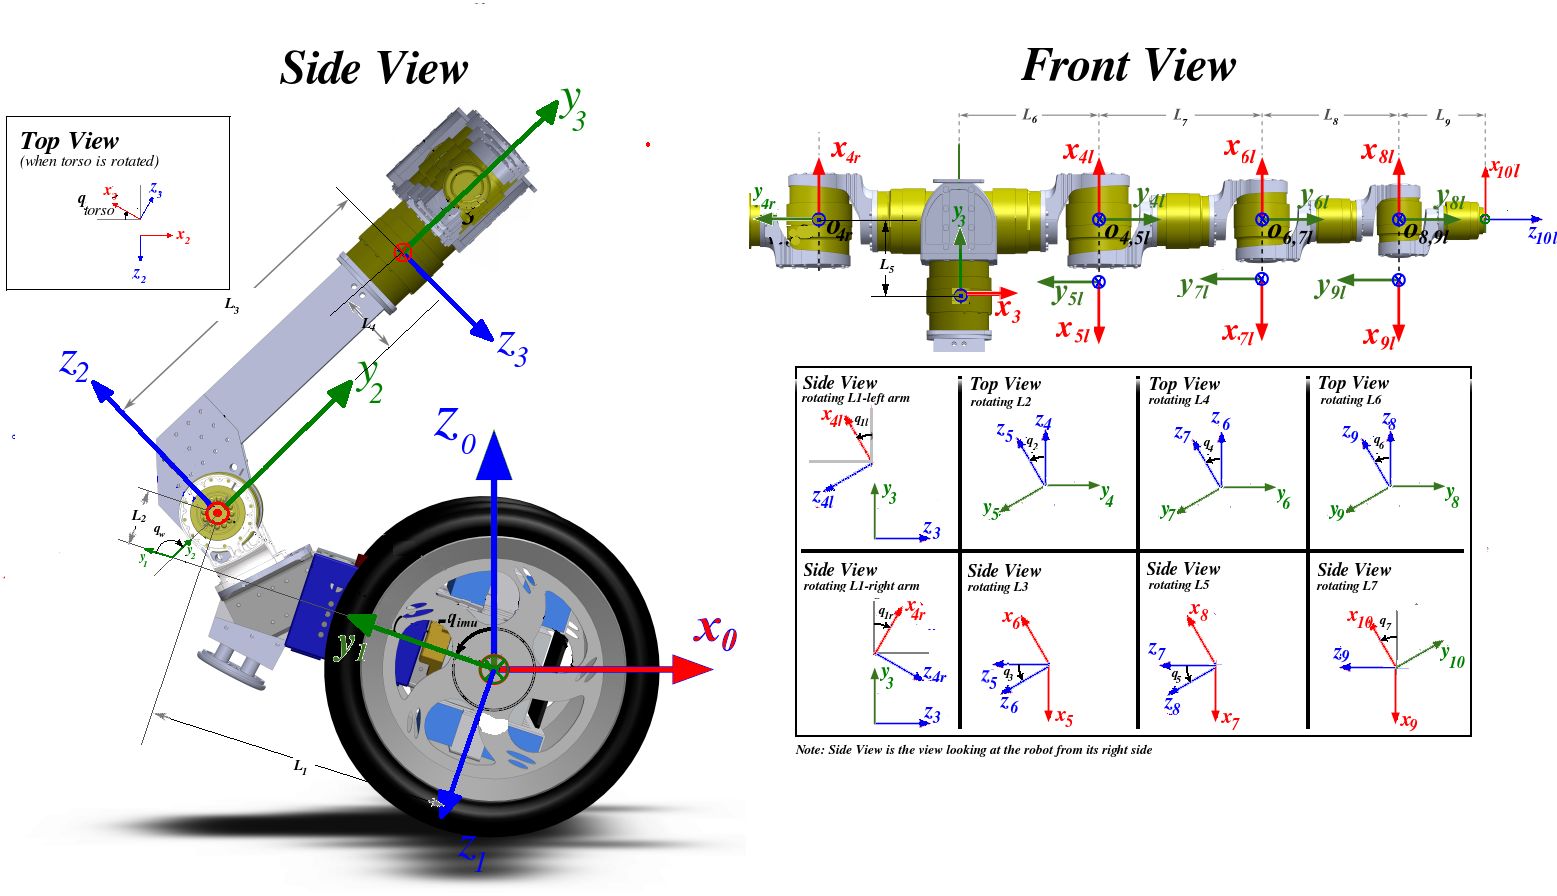
\includegraphics[width=1.0\textwidth]{Figures/framesLHRule.png}
 \caption{Frames of references on the robot}
 \label{fig:frames}
\end{figure}

We will be using the Kane's formulation. This is done so that our current analysis can easily be merged with
the dynamic modelling of wheeled inverted pendulum which is found in terms of quais-velocities, that prohibit
the use of Lagrange for analytical modelling of the robot. Kane's method however is applicable for this
problem.

\section{Introduction to Kane's Formulation}
\begin{align}
 \sum_{\substack{k}} \left[ m_k \bar{a}_{Gk} \cdot \left(\bar{v}_{Gk}\right)_j + \left( \frac{d\bar{H}_{Gk}}{dt} 
 \right) \cdot \left( \bar\omega_k \right)_j \right] = \sum_{\substack{n}}  \bar{F}_n \cdot \left( \bar{v}_n \right)_j 
 + \sum_{\substack{n}}  \bar{M}_m \cdot \left( \bar{\omega}_m \right)_j \;\; j=1 ... K
\end{align}
where 
\begin{itemize}[label={}]
\item[$j$] is the unique number identifyin each generalized co-ordinate in the system
\item[$k$] is the unique number identifying each rigid body in the system
\item[$n$] is the unique number identifying each external force acting on the system
\item[$m$] is the unique number identifying each external torque acting on the system
\item[$m_k$] is the mass of the $k$th body
\item[$\bar{a}_{Gk}$] is the acceleration of the center of mass of $k$th body
\item[$\bar{v}_{Gk}$] is the velocity of the center of mass of the $k$th body
\item[$\bar{H}_{Gk}$] is the angular momentum of body $k$ about its center of mass
\item[$\bar{\omega}_{k}$] is the angular velocity of the body $k$
\item[$F_n$] is the $n$th external force
\item[$M_m$] is the $m$th external moment
\item[$\bar{v}_{n}$] is the velocity of the point at which external Force $F_n$ is acting
\item[$\bar{\omega}_{m}$] is the angular velocity of the body on which torque is acting relative to the actuator applying the torque
\item[$()_j$] $=\frac{\partial ()}{\partial \dot{q}_j}$ the partial derivative of the quantity in brackets $()$ with respect to the generalized
velocity $\dot{q}_j$
\end{itemize}
% The Lagrange formulation describes the behavior of a dynamic system in terms of work and energy stored in the
% system. The Lagrange equations are commonly written in the form:
% \begin{align}
%  &\Gamma_i = \frac{d}{dt}\frac{\partial L}{\partial \dot{q}_i}-\frac{\partial L}{\partial q_i} \quad for i \in \mathbb{F} \label{eq:Lagrange}
% \end{align} where $L$ is the Lagrangian of the robot defined as the difference berween the kinetic energy $E$ and potential 
% energy $U$ of the system:
% \[
%  L = E-U
% \]
% \subsection{General Form of the Dynamic Equations}
% The kinetic energy of the system is a quadratic function in the joint velocities such that:
% \begin{align}
%  &E = \frac{1}{2}\mathbf{\dot{q}^TA\dot{q}}
% \end{align} where $\mathbf{A}$ is the $n\times n$ symmetric and positive definite \textit{inertia matrix} of the robot.
% Its elements are functions of the joint positions. The $(i,j)$ element of $\mathbf{A}$ is denoted $A_{ij}$. Since the 
% potential energy is a function of the joint positions, equation \ref{eq:Lagrange} leads to:
% \begin{align}
%  &\mathbf{\Gamma=A(q)\ddot{q}+C(q,\dot{q})\dot{q}+Q(q)}
% \end{align} where:
% \begin{itemize}
%  \item $\mathbf{C(q,\dot{q})\dot{q}}$ is the $n\times 1$ vector of Coriolis and centrifugal torques, such that: 
%  $\mathbf{C\dot{q} = \dot{A}\dot{q}}-\frac{\partial E}{\partial \mathbf{q}}$
%  \item $\mathbf{Q} = \left[\begin{matrix} Q_1 & Q_2 & Q_3 & Q_{4l} & ... & Q_{10l} & Q_{4r} & ... & Q_{10r} \end{matrix} \right]^T$ 
%  is the vector of gravity torques
% \end{itemize}
% So the dynamic model of a tree-structured robot is described by $n$ coupled and nonlinear second order differential
% equations. The elements of $\mathbf{A}$, $\mathbf{C}$ and $\mathbf{Q}$ are functions of geometric and inertial 
% parameters of the robot.
 
% \subsection{Computation of the elements of $\mathbf{A}$, $\mathbf{C}$ and $\mathbf{Q}$}
% To compute the elements of $\mathbf{A}$, $\mathbf{C}$ and $\mathbf{Q}$, we begin by symbollically computing the 
% expressions of the kinetic and potential energies of all the links of the robot. Then we proceed as follows:
%  \begin{itemize}
%   \item the elements $A_{ij}$ is equal to the coefficient of $\left(\frac{\dot{q}_i^2}{2}\right)$ in the expression of
%   the kinetic energy, while $A_{ij}$, for $i \neq j$, is equal to the coefficient of $\dot{q}_i\dot{q}_j$
%   \item for calculating the elements of $\mathbf{C}$, there exist several forms of the vector $\mathbf{C(q,\dot{q})\dot{q}}$.
%  Using the \textit{Christoffell symbols} $c_{i,jk}$, the $(i,j)$ elements of the matrix $\mathbf{C}$ can be written as:
%  \begin{align}
%   \begin{cases}
%    C_{ij} = \sum\limits^{n}_{k=1}c_{i,jk}\dot{q}_k \\
%    c_{i,jk} = \frac{1}{2}\left[\frac{\partial A_{ij}}{\partial q_k} + \frac{\partial A_{ik}}{\partial q_j} - \frac{\partial A_{jk}}{\partial q_i}\right]
%   \end{cases}
%  \end{align}
%  \item The $Q_i$ element of the vector $\mathbf{Q}$ is calculated according to:
%  \begin{align}
%   Q_i = \frac{\partial U}{\partial q_i}
%  \end{align}
%  \end{itemize}

\section{Finding Dynamic Model for our robot}
In this section we determine the symbolic expression for the  total kinetic energy $E$ of the robot.

\subsection{Transformations}

The transformation of frame $R_i$ into frame $R_j$ is represented by the homogeneous transformation matrix
${}^{i}T_j$ such that.
\begin{align}
 {}^{i}T_j = \left[\begin{matrix}{}^{i}s_j & {}^{i}n_j & {}^{i}a_j & {}^{i}P_j \end{matrix} \right] 
  = \left[\begin{matrix} & {}^iA_j & & {}^iP_j \\ 0 & 0 & 0 & 1 \end{matrix}\right]
  = \left[\begin{matrix}s_x & n_x & a_x & P_x  \\ s_y & n_y & a_y & P_y 
  \\ s_z & n_z & a_z & P_z \\ 0 & 0 & 0 & 1 \end{matrix} \right]
\end{align}
where ${}^is_j$, ${}^in_j$ and ${}^ia_j$ contain the components of the unit vectors along the $x_j$, 
$y_j$ and $z_j$ axes respectively expressed in frame $R_i$, and where ${}^iP_j$ is the vector representing
the coordinates of the origin of frame $R_j$ expressed in frame $R_i$.

The transformation matrix ${}^iT_j$ can be interpreted as: (a) the transformation from frame $R_i$ to frame $R_j$
and (b) the representation of frame $R_j$ with respect to frame $R_i$. Using figure \ref{fig:frames}, we can
write down these transformation matrices for our system as follows:

\[
 \scalemath{0.75}{{}^0T_1 = \left[\begin{matrix} 0 & sq_{imu} & -cq_{imu} & 0 \\ -1 & 0 & 0 & 0 \\ 0 & cq_{imu} & sq_{imu} & 0 \\ 0 & 0 & 0 & 1 \end{matrix}\right],
 {}^1T_2 = \left[\begin{matrix} 1 & 0 & 0 & 0 \\ 0 & cq_w & sq_w & L_1 \\ 0 & -sq_w & cq_w & -L_2 \\ 0 & 0 & 0 & 1 \end{matrix}\right], 
 {}^2T_3 = \left[\begin{matrix} -cq_{torso} & 0 & sq_{torso} & 0 \\ 0 & 1 & 0 & L_3 \\ -sq_{torso} & 0 & -cq_{torso} & L_4 \\ 0 & 0 & 0 & 1 \end{matrix}\right],}
\]

\[
 \scalemath{0.75}{{}^3T_{4l} = \left[\begin{matrix} 0 & 1 & 0 & L_6 \\ cq_{1l} & 0 & -sq_{1l} & L_5 \\ -sq_{1l} & 0 & -cq_{1l} & 0 \\ 0 & 0 & 0 & 1 \end{matrix}\right], 
 {}^3T_{4r} = \left[\begin{matrix} 0 & -1 & 0 & -L_6 \\ cq_{1r} & 0 & -sq_{1r} & L_5 \\ sq_{1r} & 0 & cq_{1r} & 0 \\ 0 & 0 & 0 & 1 \end{matrix}\right], 
 {}^4T_5 = \left[\begin{matrix} -1 & 0 & 0 & 0 \\ 0 & -cq_2 & -sq_2 & 0 \\ 0 & -sq_2 & cq_2 & 0 \\ 0 & 0 & 0 & 1 \end{matrix}\right], }
\]
 
\[
 \scalemath{0.75}{ {}^5T_6 = \left[\begin{matrix} -cq_3 & 0 & sq_3 & 0 \\ 0 & -1 & 0 & -L_7 \\ sq_3 & 0 & cq_3 & 0 \\ 0 & 0 & 0 & 1 \end{matrix}\right], 
 {}^6T_7 = \left[\begin{matrix} -1 & 0 & 0 & 0 \\ 0 & -cq_4 & -sq_4 & 0 \\ 0 & -sq_4 & cq_4 & 0 \\ 0 & 0 & 0 & 1 \end{matrix}\right], 
 {}^7T_8 = \left[\begin{matrix} -cq_5 & 0 & sq_5 & 0 \\ 0 & -1 & 0 & -L_8 \\ sq_5 & 0 & cq_5 & 0 \\ 0 & 0 & 0 & 1 \end{matrix}\right], }
\]
 
\[
 \scalemath{0.75}{{}^8T_9 = \left[\begin{matrix} -1 & 0 & 0 & 0 \\ 0 & -cq_6 & -sq_6 & 0 \\ 0 & -sq_6 & cq_6 & 0 \\ 0 & 0 & 0 & 1 \end{matrix}\right], 
 {}^9T_{10} = \left[\begin{matrix} -cq_7 & -sq_7 & 0 & 0 \\ 0 & 0 & -1 & -L_9 \\ sq_7 & -cq_7 & 0 & 0 \\ 0 & 0 & 0 & 1 \end{matrix}\right] }
\]


\subsection{Velocities and Accelerations of Frames}
The angular and linear velocities of the frames can be calculated using the recursive formulation:

\begin{align}
 &{}^j\omega_j={}^jA_i{}^i\omega_i+\dot{q}_j\;{}^je_j \\
 &{}^j\alpha_j={}^jA_i{}^i\alpha_i+\ddot{q}_j\;{}^je_j+\dot{q}_j\;({}^j\omega_j \times {}^je_j) \\
 &{}^jV_j={}^jA_i\left({}^iV_i+{}^i\omega_i \times {}^iP_j\right) \\
 &{}^ja_j={}^jA_i\left({}^ia_i+{}^i\alpha_i \times {}^iP_j + {}^i\omega_i \times ({}^i\omega_i \times {}^iP_j)\right)
\end{align} where ${}^i\omega_j$, ${}^i\alpha_j$, ${}^ia_j$ and ${}^iV_j$ denote the angular velocity, linear velocity, 
angular acceleration and linear acceleration repectively of frame $j$ measured with respect to the 
world frame and represented in frame $i$. ${}^je_j$ denotes the direction of local angular velocity of frame $j$ represented in frame $j$. 
$i, j \in \mathbb{F}$ identify the frames and $i$ identifies the antecedent frame of $j$. So, the rotation ${}^jA_i$ and the 
translation ${}^jP_i$ that appear in these equations can not be directly deduced from the transformations listed in the previous section, 
as the they all represent ${}^iT_j$ (note the position of $i$ and $j$). Rather, we need to use following expressions to deduce our matrices:
\begin{align}
 &{}^jA_i = {}^iA_j^T \nonumber \\ 
 &{}^jP_i = -{}^iA_j^T\,{}^iP_j \nonumber
\end{align}

Since frame $R_0$ is fixed ${}^0\omega_0$ and ${}^0V_0$ are both $\left[\begin{matrix}0 & 0 & 0\end{matrix}\right]^T$. We can deduce directions of 
local angular velocities of the frames using figure \ref{fig:frames} as follows.

\[
\scalemath{0.75}{{}^1e_1 = \left[\begin{matrix}-1 & 0 & 0\end{matrix}\right]^T, 
{}^2e_2 = \left[\begin{matrix}-1 & 0 & 0\end{matrix}\right]^T, 
{}^3e_3 = \left[\begin{matrix}0 & -1 & 0\end{matrix}\right]^T, 
{}^4e_4 = \left[\begin{matrix}0 & -1 & 0\end{matrix}\right]^T,}
\]
\[
\scalemath{0.75}{{}^5e_5 = \left[\begin{matrix}-1 & 0 & 0\end{matrix}\right]^T, 
{}^6e_6 = \left[\begin{matrix}0 & -1 & 0\end{matrix}\right]^T, 
{}^7e_7 = \left[\begin{matrix}-1 & 0 & 0\end{matrix}\right]^T, 
{}^8e_8 = \left[\begin{matrix}0 & -1 & 0\end{matrix}\right]^T,}
\]
\[
\scalemath{0.75}{{}^9e_9 = \left[\begin{matrix}-1 & 0 & 0\end{matrix}\right]^T, 
{}^{10}e_{10} = \left[\begin{matrix}0 & 0 & -1\end{matrix}\right]^T}
\]

This information can now be used to derive expressions for the velocities and accelerations of the frames.

\subsection{Inertial Forces}
\begin{align}
 \scalemath{0.775}{\bar{v}_{Gk}}&\scalemath{0.775}{=\bar{v}_k+\bar{\omega}_k \times \bar{S}_k} \nonumber \\
 \scalemath{0.775}{\bar{a}_{Gk}}&\scalemath{0.775}{=\bar{a}_k+\bar{\alpha}_k \times \bar{S}_k + \bar{\omega}_k \times (\bar{\omega}_k \times \bar{S}_k)} \nonumber \\
 \scalemath{0.775}{\bar{H}_{Gk}}&\scalemath{0.775}{=\mathbf{J}_{Gk} \bar{\omega}_k} \nonumber \\ 
 \scalemath{0.775}{\frac{d\bar{H}_{Gk}}{dt}}&\scalemath{0.775}{=\mathbf{J}_{Gk} \bar{\alpha}_k + \bar{\omega}_k \times \mathbf{J}_{Gk} \bar{\omega}_k} \nonumber \\
 &\scalemath{0.775}{=(\mathbf{J}_{k}+m_k\mathbf{S}^{\times}_k\mathbf{S}^{\times}_k) \bar{\alpha}_k + \bar{\omega}_k \times (\mathbf{J}_{k}+m_k\mathbf{S}^{\times}_k\mathbf{S}^{\times}_k) \bar{\omega}_k} \nonumber \\
 &\scalemath{0.775}{=\mathbf{J}_{k} \bar{\alpha}_k + \bar{\omega}_k \times \mathbf{J}_{k} \bar{\omega}_k + m_k\mathbf{S}^{\times}_k\mathbf{S}^{\times}_k\bar{\alpha}_k + \bar{\omega}_k \times (m_k\mathbf{S}^{\times}_k\mathbf{S}^{\times}_k \bar{\omega}_k)} \nonumber \\
 \scalemath{0.775}{m_k \bar{a}_{Gk} \cdot \left(\bar{v}_{Gk}\right)_j} &\scalemath{0.775}{=  m_k \bar{a}_{Gk} \cdot \left(\bar{v}_k+\bar{\omega}_k \times \bar{S}_k\right)_j} \nonumber \\
 &\scalemath{0.775}{=  m_k \bar{a}_{Gk} \cdot \left(\bar{v}_k\right)_j + m_k \bar{a}_{Gk} \cdot \left(\bar{\omega}_k \times \bar{S}_k\right)_j} \nonumber \\
 &\scalemath{0.775}{=  m_k \bar{a}_{Gk} \cdot \left(\bar{v}_k\right)_j - m_k \left( \bar{a}_k+\bar{\alpha}_k \times \bar{S}_k + \bar{\omega}_k \times (\bar{\omega}_k \times \bar{S}_k) \right) \cdot \left(\bar{S}_k \times \bar{\omega}_k\right)_j} \nonumber \\
 &\scalemath{0.775}{=  m_k \bar{a}_{Gk} \cdot \left(\bar{v}_k\right)_j - m_k \left( \bar{a}_k-\bar{S}_k \times \bar{\alpha}_k - \bar{\omega}_k \times (\bar{S}_k \times \bar{\omega}_k) \right) \cdot \left(\bar{S}_k \times \left(\bar{\omega}_k\right)_j\right)} \nonumber \\
 &\scalemath{0.775}{=  m_k \bar{a}_{Gk} \cdot \left(\bar{v}_k\right)_j - m_k \left( \bar{a}_k-\mathbf{S}^{\times}_k \bar{\alpha}_k - \mathbf{\omega}^{\times}_k \mathbf{S}^{\times}_k \bar{\omega}_k \right)^T  \mathbf{S}^{\times}_k \left(\bar{\omega}_k\right)_j} \nonumber \\
 &\scalemath{0.775}{=  m_k \bar{a}_{Gk} \cdot \left(\bar{v}_k\right)_j - m_k \left( \mathbf{S}^{\times T}_k \bar{a}_k -  \mathbf{S}^{\times T}_k \mathbf{S}^{\times}_k \bar{\alpha}_k - \mathbf{S}^{\times T}_k \mathbf{\omega}^{\times}_k \mathbf{S}^{\times}_k \bar{\omega}_k \right)^T  \left(\bar{\omega}_k\right)_j} \nonumber \\
 &\scalemath{0.775}{=  m_k \bar{a}_{Gk} \cdot \left(\bar{v}_k\right)_j + m_k \left( \mathbf{S}^{\times}_k \bar{a}_k -  \mathbf{S}^{\times}_k \mathbf{S}^{\times}_k \bar{\alpha}_k - \mathbf{S}^{\times}_k \mathbf{\omega}^{\times}_k \mathbf{S}^{\times}_k \bar{\omega}_k \right)^T  \left(\bar{\omega}_k\right)_j} \nonumber \\
 &\scalemath{0.775}{=  m_k \bar{a}_{Gk} \cdot \left(\bar{v}_k\right)_j + m_k \left( \bar{S}_k \times \bar{a}_k -  \bar{S}_k \times \bar{S}_k \times \bar{\alpha}_k - \bar{S}_k \times ( \bar{\omega}_k \times ( \bar{S}_k \times \bar{\omega}_k ) ) \right) \cdot  \left(\bar{\omega}_k\right)_j} \nonumber \\
 &\scalemath{0.775}{=  m_k \bar{a}_{Gk} \cdot \left(\bar{v}_k\right)_j + m_k \left( \bar{S}_k \times \bar{a}_k -  \bar{S}_k \times \bar{S}_k \times \bar{\alpha}_k + \bar{\omega}_k \times ( ( \bar{S}_k \times \bar{\omega}_k ) \times  \bar{S}_k ) + ( \bar{S}_k \times \bar{\omega}_k ) \times ( \bar{S}_k \times \bar{\omega}_k )  \right) \cdot  \left(\bar{\omega}_k\right)_j} \nonumber \\
 &\scalemath{0.775}{=  m_k \bar{a}_{Gk} \cdot \left(\bar{v}_k\right)_j + m_k \left( \bar{S}_k \times \bar{a}_k -  \bar{S}_k \times \bar{S}_k \times \bar{\alpha}_k - \bar{\omega}_k \times ( \bar{S}_k \times ( \bar{S}_k \times \bar{\omega}_k ) ) + 0  \right) \cdot  \left(\bar{\omega}_k\right)_j} \nonumber \\
 &\scalemath{0.775}{=  m_k \bar{a}_{Gk} \cdot \left(\bar{v}_k\right)_j + \left( m_k \bar{S}_k \times \bar{a}_k -  m_k \mathbf{S}^{\times}_k \mathbf{S}^{\times}_k \bar{\alpha}_k - \bar{\omega}_k \times (m_k \mathbf{S}^{\times}_k \mathbf{S}^{\times}_k \bar{\omega}_k) \right) \cdot  \left(\bar{\omega}_k\right)_j} \nonumber \\
 \scalemath{0.775}{m_k \bar{a}_{Gk} \cdot \left(\bar{v}_{Gk}\right)_j} &\scalemath{0.775}{ + \left( \frac{d\bar{H}_{Gk}}{dt} \right) \cdot \left( \bar\omega_k \right)_j} \nonumber \\
 &\scalemath{0.775}{=  m_k \bar{a}_{Gk} \cdot \left(\bar{v}_k\right)_j + \left( m_k \bar{S}_k \times \bar{a}_k -  m_k \mathbf{S}^{\times}_k \mathbf{S}^{\times}_k \bar{\alpha}_k - \bar{\omega}_k \times (m_k \mathbf{S}^{\times}_k \mathbf{S}^{\times}_k \bar{\omega}_k) \right) \cdot  \left(\bar{\omega}_k\right)_j} \nonumber \\
 &\scalemath{0.775}{\hspace{40pt}+\left(\mathbf{J}_{k} \bar{\alpha}_k + \bar{\omega}_k \times \mathbf{J}_{k} \bar{\omega}_k + m_k\mathbf{S}^{\times}_k\mathbf{S}^{\times}_k\bar{\alpha}_k + \bar{\omega}_k \times (m_k\mathbf{S}^{\times}_k\mathbf{S}^{\times}_k \bar{\omega}_k)\right) \cdot \left( \bar\omega_k \right)_j} \nonumber \\
 &\scalemath{0.775}{=  m_k \bar{a}_{Gk} \cdot \left(\bar{v}_k\right)_j + \left( m_k \bar{S}_k \times \bar{a}_k + \mathbf{J}_{k} \bar{\alpha}_k + \bar{\omega}_k \times \mathbf{J}_{k} \bar{\omega}_k\right) \cdot  \left(\bar{\omega}_k\right)_j} \nonumber 
\end{align}

% \subsection{Kinetic Energy}
% The kinetic energy of the robot is given as:
% \begin{align}
%  &E = \sum_{\substack{j \in \mathbb{F}}} E_j
% \end{align}where $E_j$ denotes the kinetic energy of link $j$, which can be computed by
% \begin{align}
%  &E_j = \frac{1}{2}(\omega_j^TI_{Gj}\omega_j+M_jV_{Gj}^TV_{Gj}) \label{eq:KE1}
% \end{align} where the velocity of the center of mass can be expressed as:
% \[
%  V_{Gj} = V_j + \omega_j \times S_j
% \] and since:
% \[
%  J_j = I_{Gj} - M_j \hat{S}_j \hat{S_j}
% \] equation \ref{eq:KE1} becomes:
% \begin{align}
%  &E_j = \frac{1}{2}(\omega_j^TJ_{Gj}\omega_j+M_jV_j^TV_j + 2\mathbf{MS}_j^T(V_j \times \omega_j)) \label{eq:KE2}
% \end{align} See section \ref{sec:expressionKE} in the appendix to know the details of the derivation.

\subsection{Potential Energy}
The total potential energy $U$ of the robot is given by:
\begin{align}
 U = \sum_{\substack{j \in \mathbb{F}}} U_j = \sum_{\substack{j \in \mathbb{F}}} -M_j \mathbf{g}^T(L_{0,j}+S_j) \label{eq:PE1}
\end{align}
where $L_{0,j}$ is the position vector from the origin $O_0$ to $O_j$ and $\mathbf{g}$ is the gravitatonal acceleration. Projecting 
the vectors appearing in \ref{eq:PE1} into frame $R_0$, we obtain:
\begin{align}
 U_j &= -M_j\,{}^0\mathbf{g}^T({}^0P_j+{}^0A_j\,{}^jS_j) \\ &= -{}^0\mathbf{g}^T(M_j\,{}^0P_j+{}^0A_j\,{}^j\mathbf{MS}_j) \\ 
 &= -\left[\begin{matrix} {}^0\mathbf{g}^T && 0 \end{matrix} \right] {}^0T_j\left[ \begin{matrix} {}^j\mathbf{MS}_j \\ M_j \end{matrix} \right]
\end{align}
Given the frames defined in figure \ref{fig:frames}, ${}^0\mathbf{g} = \left[\begin{matrix}0 & 0 & -g \end{matrix}\right]^T$.

% \section{Effects of forces and torques on the end effectors}
% 
% The well known relationship between joint torques and end effector forces on a simple serial robot is:
% \[
%  \mathbf{\Gamma} = \mathbb{J}_n^T\mathbbm{f}_{e@n}
% \] where
% \begin{itemize}
%  \item $\mathbf{\Gamma}$ is the vector of torques of the individual joints in the chain
%  \item $\mathbbm{f}_{e@n} = \left[ \begin{matrix} f_{e@n} \\ \tau_{e@n} \end{matrix} \right]$ is the wrench applied by the robot at
%  the origin of the $n$th frame (i.e. the last link in the chain which has the end-effector mounted on it). This wrench is usually
%  represented in frame $R_n$ or in the world frame $R_0$ denoted as ${}^n\mathbbm{f}_{e@n}$ or ${}^0\mathbbm{f}_{e@n}$ respectively.
%  \item $\mathbb{J}_n$ is $6 \times n$ Jacobian matrix of the robot calculated using:
%  \[
%    \mathbb{J}_n = \left[ \begin{matrix} e_1\times L_{1,n} & ... & e_n\times L_{n,n} \\ e_1 & ... & e_n \end{matrix} \right]
%  \] where $e_j$ denotes the unit vectors along the local angular velocities of the frame $j$ and $L_{j,n}$ is the
%  position vector from $O_j$ to $O_n$. These vectors are expressed in the same frame as the wrench $\mathbbm{f}_{e@n}$.
%  So for ${}^0\mathbbm{f}_{e@n}$ all vectors in the Jacobian matrix will be expressed in frame $0$ and the Jacobian will
%  be denoted as ${}^0\mathbb{J}_n$. Similarly for ${}^n\mathbbm{f}_{e@n}$ the Jacobian will be denoted ${}^n\mathbb{J}_n$.
% \end{itemize}
% 
% \subsection{Jacobians for the two-armed robot}
% For the case of krang, we will have two wrenches $\mathbbm{f}_{el@10l}$ and $\mathbbm{f}_{er@10r}$ applied at 
% two end-effectors on the right and the left arms respectively. As previously $el$ and $er$ are identifying the
% wrench and $10l$ and $10r$ are idenfying the frames at whose origin the wrenches are being applied. The joint
% torques will now be calculated using the equation:
% \begin{align}
%  \mathbf{\Gamma} = \mathbb{J}_{10l}^T\mathbbm{f}_{el@10l} + \mathbb{J}_{10r}^T\mathbbm{f}_{er@10r}
% \end{align} where
% \begin{itemize}
%  \item $\mathbf{\Gamma} = \left[ \begin{matrix} \tau_1 & \tau_2 & \tau_3 & \tau_{4l} & ... & \tau_{10l} & \tau_{4r} & ... & \tau_{10r} \end{matrix} \right]^T$
%  \item $\scalemath{0.775}{\mathbb{J}_{10l} = \left[ \begin{matrix} e_1\times L_{1,10l} & e_2\times L_{2,10l} 
%  & e_3\times L_{3,10l} & e_{4l}\times L_{4l,10l} & ... & e_{10l}\times L_{10l,10l} & O_{3\times 7} \\ 
%  e_1 & e_2 & e_3 & e_{4l} & ... & e_{10l} & O_{3\times 7} \end{matrix} \right]}$
%  \item $\scalemath{0.75}{\mathbb{J}_{10r} = \left[ \begin{matrix} e_1\times L_{1,10r} & e_2\times L_{2,10r} 
%  & e_3\times L_{3,10r} & O_{3\times 7} & e_{4r}\times L_{4r,10r} & ... & e_{10r}\times L_{10r,10r} \\ 
%  e_1 & e_2 & e_3 & O_{3\times 7} & e_{4r} & ... & e_{10r}  \end{matrix} \right]}$
% \end{itemize}
% 
% 
% \section{Other terms in the Lagrange Equations}
% 
% \subsection{Considering Friction}
% The most often employed model for friction is composed of Coulomb friction together with viscous friction. Therefor, the
% friction torque at joint $i$ is written as:
% \[
%  \Gamma_{fi} = F_{ci}sign(\dot{q}_i)+F_{vi}\dot{q}_i
% \]
% To take into account the friction in the dynamic model of a robot we add the vector $\mathbf{\Gamma}_f$ to the right
% side of the Lagrange equation (i.e. the vector of generalized forces), such that:
% \begin{align}
%  \mathbf{\Gamma}_f = \mathbf{diag(\dot{q})F_v+diag[sign(\dot{q}]F_c}
% \end{align} where
% \begin{itemize}
%  \item $\mathbf{F}_v = \left[\begin{matrix} F_{v1} & F_{v2} & F_{v3} & F_{v4l} & ... & F_{v10l} & F_{v4r} & ... & F_{v10r} \end{matrix}\right]^T$
%  \item $\mathbf{F}_c = \left[\begin{matrix} F_{c1} & F_{c2} & F_{c3} & F_{c4l} & ... & F_{c10l} & F_{c4r} & ... & F_{c10r} \end{matrix}\right]^T$
%  \item $\mathbf{diag(\dot{q})} is the diagonal matrix whose elements are the components of \mathbf{\dot{q}}$
% \end{itemize}
% 
% \subsection{Considering rotor inertia}
% The kinetic energy of the rotor (and transmission system) and actuator $j$, is given by the expression 
% $\frac{1}{2}I_{aj}\dot{q}_j^2$. The inertial parameter $I_{aj}$ denotes the equivalent inertia referred to the
% joint velocity. It is given by:
% \begin{align}
%  I_{aj} = N_j^2J_{mj}
% \end{align} where $J_{mj}$ is the moment of inertia of the rotor and transmissions of actuator $j$, $N_j$
% is the transmission ratio of the joint axis, equal to $\frac{\dot{q}_{mj}}{\dot{q}_j}$ where $\dot{q}_{mj}$
% denotes the rotor velocity of actuator $j$. In the case of a prismatic joint, $I_{aj}$ is an equivalent mass.
% 
% In order to consider the rotor inertia in the dynamic model of the robot, we add the inertia (or mass) $I_{aj}$
% to the $A_{jj}$ element of the matrix $\mathbf{A}$.




\bibliographystyle{plain}
\bibliography{reference}

\appendix
\section{Expression for Kinetic Energy} \label{sec:expressionKE}
We show here how the equation \ref{eq:KE2} was derived from \ref{eq:KE1}. Equation \ref{eq:KE1} is:
\begin{align}
 &E_j = \frac{1}{2}(\omega_j^TI_{Gj}\omega_j+M_jV_{Gj}^TV_{Gj}) \label{eq:appKE}
\end{align} where the velocity of the center of mass can be expressed as:
\[
 V_{Gj} = V_j + \omega_j \times S_j
\] and since:
\[
 J_j = I_{Gj} - M_j \hat{S}_j \hat{S}_j^T
\] So equation \ref{eq:appKE} becomes:
\begin{align*}
 E_j = \frac{1}{2}(\omega_j^T&(J_j + M_j \hat{S}_j \hat{S}_j)\omega_j+M_j(V_j + \omega_j \times S_j)^T(V_j + \omega_j \times S_j)) \\
 E_j = \frac{1}{2}(\omega_j^T&J_j\omega_j+M_jV_j^TV_j+ \omega_j^TM_j\hat{S}_j\hat{S}_j\omega_j+M_jV_j^T(\omega_j\times S_j) \nonumber \\
 &+ M_j(\omega_j \times S_j)^TV_j+M_j(\omega_j \times S_j)^T(\omega_j \times S_j)) 
\end{align*} Noting that the last term:
\begin{align*}
 M_j(\omega_j \times S_j)^T(\omega_j \times S_j) &= (-)(-)M_j(S_j \times \omega_j)^T(S_j \times \omega_j) \\ &= M_j(\hat{S}_j\omega_j)^T(\hat{S}_j\omega_j) \\ &= M_j\omega_j^T\hat{S}_j^T\hat{S}_j\omega_j \\ &= -M_j\omega_j^T\hat{S}_j\hat{S}_j\omega_j
\end{align*} cancels out the third term. And noting that the fourth and fifth terms are equal, we are left with:
\begin{align*}
 &E_j = \frac{1}{2}(\omega_j^TJ_j\omega_j+M_jV_j^TV_j+ 2M_j(\omega_j\times S_j)^TV_j) 
\end{align*} The last term in the above expression can be simplified as follows:
\begin{align*}
 M_j(\omega_j\times S_j)^TV_j &= M_j(\hat{\omega}_jS_j)^TV_j \\ &= M_jS_j^T\hat{\omega}_j^TV_j \\ &= -M_jS_j^T\hat{\omega}_jV_j \\ &= -M_jS_j^T(\omega_j \times V_j) \\ &= \mathbf{MS}_j^T(V_j \times \omega_j)
\end{align*} so we end up with:
\[
 E_j = \frac{1}{2}(\omega_j^TJ_{Gj}\omega_j+M_jV_j^TV_j + 2\mathbf{MS}_j^T(V_j \times \omega_j))
\]


\section{Comparison with Lagrange}
When we compare the result of Kane's method to that of Lagrange's method it turns out that there are significant differences.
Since the two systems of equations involve hundreds of variables that makes it too complex to compare the two results, we
only perform dynamic analysis on a two-link robot. The resulting systems of equation are as follows:

\subsection{Lagrange}
\begin{align}
  \mathbf{A} &= \left[ \begin{matrix} 
  \mathbf{XX}_1 + \mathbf{XX}_2 + 2 \mathbf{MY}_2 \mathbb{M}_4 + 2 \mathbf{MZ}_2 \mathbb{M}_3 + m_2 \mathbb{M}_4^2  + m_2 \mathbb{M}_3^2 &  \mathbb{M}_1 \\
  \mathbb{M}_1 &                           \mathbf{XX}_2  
  \end{matrix} \right]  \\
 \mathbf{C} &= \left[ \begin{matrix}
    \dot{q}_w \mathbb{M}_2 &  \dot{q}_w \mathbb{M}_2 + \dot{q}_{imu} \mathbb{M}_2  \\
   -\dot{q}_{imu} \mathbb{M}_2 &          0        
 \end{matrix} \right]   \\
 \mathbf{Q} &= \left[ \begin{matrix}
  \mathbf{MZ}_1 g cosq_{imu} - \mathbf{MY}_1 g sinq_{imu} + \mathbf{MZ}_2 g \mathbb{M}_5 - \mathbf{MY}_2 g \mathbb{M}_6 - g m_2 (L_2 cosq_{imu} + L_1 sinq_{imu})   \\
                                          \mathbf{MZ}_2 g \mathbb{M}_5 - \mathbf{MY}_2 g \mathbb{M}_6                                          
 \end{matrix} \right]   \\ 
\end{align}
where
\begin{itemize}[label={}]
 \item[$\mathbb{M}_1$] $= \mathbf{XX}_2 + \mathbf{MY}_2 \mathbb{M}_4 + \mathbf{MZ}_2 \mathbb{M}_3$
 \item[$\mathbb{M}_2$] $= \mathbf{MZ}_2 \mathbb{M}_4 - \mathbf{MY}_2 \mathbb{M}_3$
 \item[$\mathbb{M}_3$] $= -L_2 cos(q_w) + L_1 sin(q_w)$
 \item[$\mathbb{M}_4$] $= L_1 cos(q_w) + L_2 sin(q_w)$
 \item[$\mathbb{M}_5$] $= cosq_{imu} cosq_w - sinq_{imu} sinq_w)$
 \item[$\mathbb{M}_6$] $= cosq_{imu} sinq_w + cosq_w sinq_{imu})$
\end{itemize}

\subsection{Kane's}
\begin{align}
  \mathbf{A} &= \left[ \begin{matrix} 
   \mathbb{XX}_1 + \mathbb{XX}_2 + 2 \mathbf{MY}_2 \mathbb{M}_4 + 2 \mathbf{MZ}_2 \mathbb{M}_3 + m_2 \mathbb{M}_4^2 + m_2 \mathbb{M}_3^2 & \mathbb{M}_1  \\
        \mathbb{M}_1   &                                                      \mathbb{XX}_2  
  \end{matrix} \right]  \\
 \mathbf{C} &= \left[ \begin{matrix}
  \dot{q}_w \mathbb{M}_2  & \dot{q}_w \mathbb{M}_2 + \dot{q}_{imu} \mathbb{M}_2  \\
                  -\dot{q}_{imu} \mathbb{M}_2              &                       0                              
 \end{matrix} \right]  \\
 \mathbf{Q} &= \left[ \begin{matrix}
  \mathbf{MZ}_1 g cosq_{imu} - \mathbf{MY}_1 g sinq_{imu} + \mathbf{MZ}_2 g \mathbb{M}_5 - \mathbf{MY}_2 g \mathbb{M}_6  - g m_2 (L_2 cosq_{imu} + L_1 sinq_{imu}) \\
                                                          \mathbf{MZ}_2 g \mathbb{M}_5 - \mathbf{MY}_2 g \mathbb{M}_6                                                          
 \end{matrix} \right]  
\end{align}
where
\begin{itemize}[label={}]
 \item[$\mathbb{XX}_1$] $= \mathbf{XX}_1 + \frac{\mathbf{MY}_1^2}{m_1} + \frac{\mathbf{MZ}_1^2}{m_1}$
 \item[$\mathbb{XX}_2$] $= \mathbf{XX}_2 + \frac{\mathbf{MY}_2^2}{m_2} + \frac{\mathbf{MZ}_2^2}{m_2}$
 \item[$\mathbb{M}_1$] $= \mathbb{XX}_2 + \mathbf{MY}_2 \mathbb{M}_4 + \mathbf{MZ}_2 \mathbb{M}_3$
 \item[$\mathbb{M}_2$] $= \mathbf{MZ}_2 \mathbb{M}_4 - \mathbf{MY}_2 \mathbb{M}_3 $
 \item[$\mathbb{M}_3$] $= - L_2 cosq_w + L_1 sinq_w$
 \item[$\mathbb{M}_4$] $=  L_1 cosq_w + L_2 sinq_w$
 \item[$\mathbb{M}_5$] $= cosq_{imu} cosq_w - sinq_{imu} sinq_w$
 \item[$\mathbb{M}_6$] $= cosq_{imu} sinq_w + cosq_w sinq_{imu}$
\end{itemize}
\end{document}
